\documentclass[tikz,border=10pt]{standalone}
\usetikzlibrary{arrows.meta}

\begin{document}
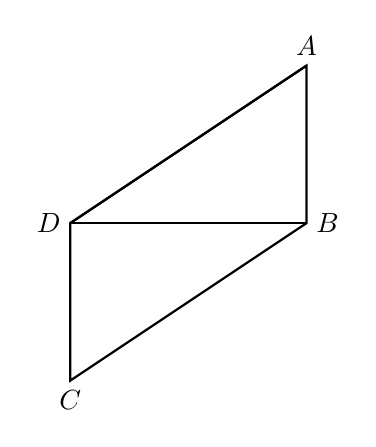
\begin{tikzpicture}
    % 定义关键点坐标
    \coordinate (B) at (0,0);
    \coordinate (A) at (0,2);
    \coordinate (D) at (-3,0);
    \coordinate (C) at (-3,-2);

    % 绘制图形边界
    \draw[thick] (A) -- (B) -- (C) -- (D) -- cycle; % 外部轮廓
    \draw[thick] (A) -- (D); % 连接 A 与 D 的斜线
    \draw[thick] (B) -- (D);


    % 标记各个顶点
    \node[above] at (A) {$A$};
    \node[right] at (B) {$B$};
    \node[below] at (C) {$C$};
    \node[left] at (D) {$D$};

\end{tikzpicture}
\end{document}